\documentclass[tikz, margin=3mm]{standalone}
\usetikzlibrary{chains, decorations.pathreplacing, positioning} 
% \usepackage[subpreambles=true]{standalone}
% \usepackage[utf8]{inputenc}
% \usepackage[english]{babel}
% \usepackage{import}
\usepackage{ifthen}
\usepackage{pgffor}
% \usetikzlibrary{chains, decorations.pathreplacing, positioning}
% \usepackage[dvipsnames]{xcolor}
\definecolor{tab10blue}{RGB}{31, 119, 180}
\definecolor{tab10orange}{RGB}{255, 127, 14}
\definecolor{tab10green}{RGB}{44, 160, 44}
\definecolor{tab10red}{RGB}{214, 39, 40}
\definecolor{tab10purple}{RGB}{148, 103, 189}
\definecolor{tab10brown}{RGB}{140, 86, 75}
\definecolor{tab10pink}{RGB}{227, 119, 194}
\definecolor{tab10gray}{RGB}{127, 127, 127}
\definecolor{tab10olive}{RGB}{188, 189, 34}
\definecolor{tab10cyan}{RGB}{23, 190, 207}
\definecolor{myBlue}{RGB}{0, 157, 248}
\definecolor{myRed}{RGB}{255, 96, 96}
\definecolor{myGreen}{RGB}{21, 173, 87}
\definecolor{darkB}{RGB}{26, 78, 102}
\definecolor{lightB}{RGB}{166, 212, 241}
\definecolor{darkG}{RGB}{38, 133, 120}
\tikzset{%
    node distance = 22mm,
    every neuron/.style={
        circle,
        draw,
        minimum size=17pt,
        inner sep=0pt,
    },
    neuron -1/.style={
        draw=none, 
        scale=4,
        text height=0.333cm,
        execute at begin node=\color{black}$\vdots$
    },
    annot/.style = {text width=4em, text centered, node distance = 6mm},
    B/.style args = {#1/#2}{%B: Brace
        decorate,
        decoration={brace, amplitude=5pt,
                    pre=moveto,pre length=1pt,post=moveto,post length=1pt,
                    raise=#1,
                    #2,% for mirroring of brace
                    },
    thick},
}
\begin{document}
\pagestyle{empty}

\def\layersep{2.5cm}

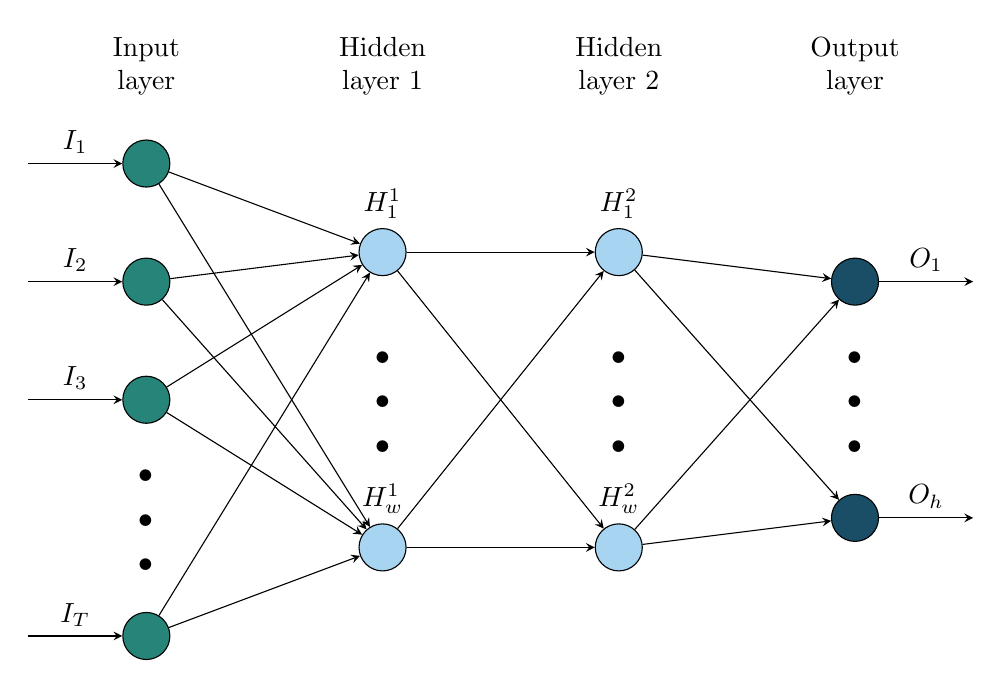
\begin{tikzpicture}[x=1.5cm, y=1.5cm, >=stealth]
    \foreach \m/\l [count=\y] in {1,2,3,-1,4}{
        \ifthenelse{\m > 0}
            {\node [every neuron/.try, neuron \m/.try, fill=darkG ] (input-\m) at (0,2.5-\y) {};}
            {\node [every neuron/.try, neuron \m/.try] (input-\m) at (0,2.5-\y) {};};
    }
    

    \foreach \m [count=\y] in {1,-1,2}{
        \ifthenelse{\m > 0}
            {\node [every neuron/.try, neuron \m/.try, fill=lightB ] (hidden1-\m) at (2,2-\y*1.25) {};}
            {\node [every neuron/.try, neuron \m/.try] (hidden1-\m) at (2,2-\y*1.25) {};};
    }

    
    \foreach \m [count=\y] in {1,-1,2}{
        \ifthenelse{\m > 0}
            {\node [every neuron/.try, neuron \m/.try, fill=lightB ] (hidden2-\m) at (4,2-\y*1.25) {};}
            {\node [every neuron/.try, neuron \m/.try] (hidden2-\m) at (4,2-\y*1.25) {};};
    }

    \foreach \m [count=\y] in {1,-1,2} {
        \ifthenelse{\m > 0}
            {\node [every neuron/.try, neuron \m/.try, fill=darkB] (output-\m) at (6,1.5-\y) {};}
            {\node [every neuron/.try, neuron \m/.try] (output-\m) at (6,1.5-\y) {};};
    }
    
    
\foreach \l [count=\i] in {1,2,3,T}
  \draw [<-] (input-\i) -- ++(-1,0)
    node [above, midway] {$I_\l$};

\foreach \l [count=\i] in {1,w}
  \node [above] at (hidden1-\i.north) {$H^1_\l$};

\foreach \l [count=\i] in {1,w}
  \node [above] at (hidden2-\i.north) {$H^2_\l$};

\foreach \l [count=\i] in {1,h}
  \draw [->] (output-\i) -- ++(1,0)
    node [above, midway] {$O_\l$};

\foreach \i in {1,...,4}
  \foreach \j in {1,...,2}
    \draw [->] (input-\i) -- (hidden1-\j);

\foreach \i in {1,...,2}
  \foreach \j in {1,...,2}
    \draw [->] (hidden1-\i) -- (hidden2-\j);

\foreach \i in {1,...,2}
  \foreach \j in {1,...,2}
    \draw [->] (hidden2-\i) -- (output-\j);

\node [align=center, above] at (0,2) {Input \\ layer};
\node [align=center, above] at (2,2) {Hidden \\ layer 1};
\node [align=center, above] at (4,2) {Hidden \\ layer 2};
\node [align=center, above] at (6,2) {Output \\ layer};
% \foreach \l [count=\x from 0] in {Input, $\textrm{Hidden}^{1}$, $\textrm{Hidden}^{2}$, Ouput}
%   \node [align=center, above] at (\x*2,2) {\l \\ layer};


\end{tikzpicture}
% End of code
\end{document}